\section{开始撰写论文}
\subsection{施工流向、程序及顺序}
\subsubsection{施工流向}
\subsubsection{施工程序}
\subsubsection{施工顺序}

\subsection{施工组织机构及主要管理人员职能}
\subsubsection{施工组织机构}

本工程拟实行项目法施工管理,委派实践经验丰富和管理水平高的同志担任项目部主要负责人,选聘技术、管理水平高的技术人员、管理人员、专业工长组建项目部。

项目管理层由项目经理、项目副经理、技术负责人、安全主管、质量主管、材料主管、保卫主管、机械主管和后勤主管等成员组成,
在建设单位、监理单位和公司的指导下,负责对本工程的工期、质量、安全、成本等实施计划。组织、协调、控制和决策,对各生产施工要素实施全过程的动态管理。

项目经理部对工程项目进行计划管理。计划管理主要体现在工程项目综合进度计划和经济计划。

作业层人员的配备:施工人员均挑选有丰富施工经验和劳动技能的正式工和合同工,分工种组成作业班组,挑选技术过硬、思想素质好的正式职工带班。

为保证项目部管理层指令畅通有效,工作安排采用“施工任务书”的形式。要求签发人和执行人签字,项目经理层作为执行的监督者。
施工任务书的工作内容完成后由签发人封闭并签字,如未能封闭必须找出原因并对执行人进行处罚。

项目经理部组织机构图见 \ref{fig:c2f1}

\begin{figure}[thbp!]
    \centering
    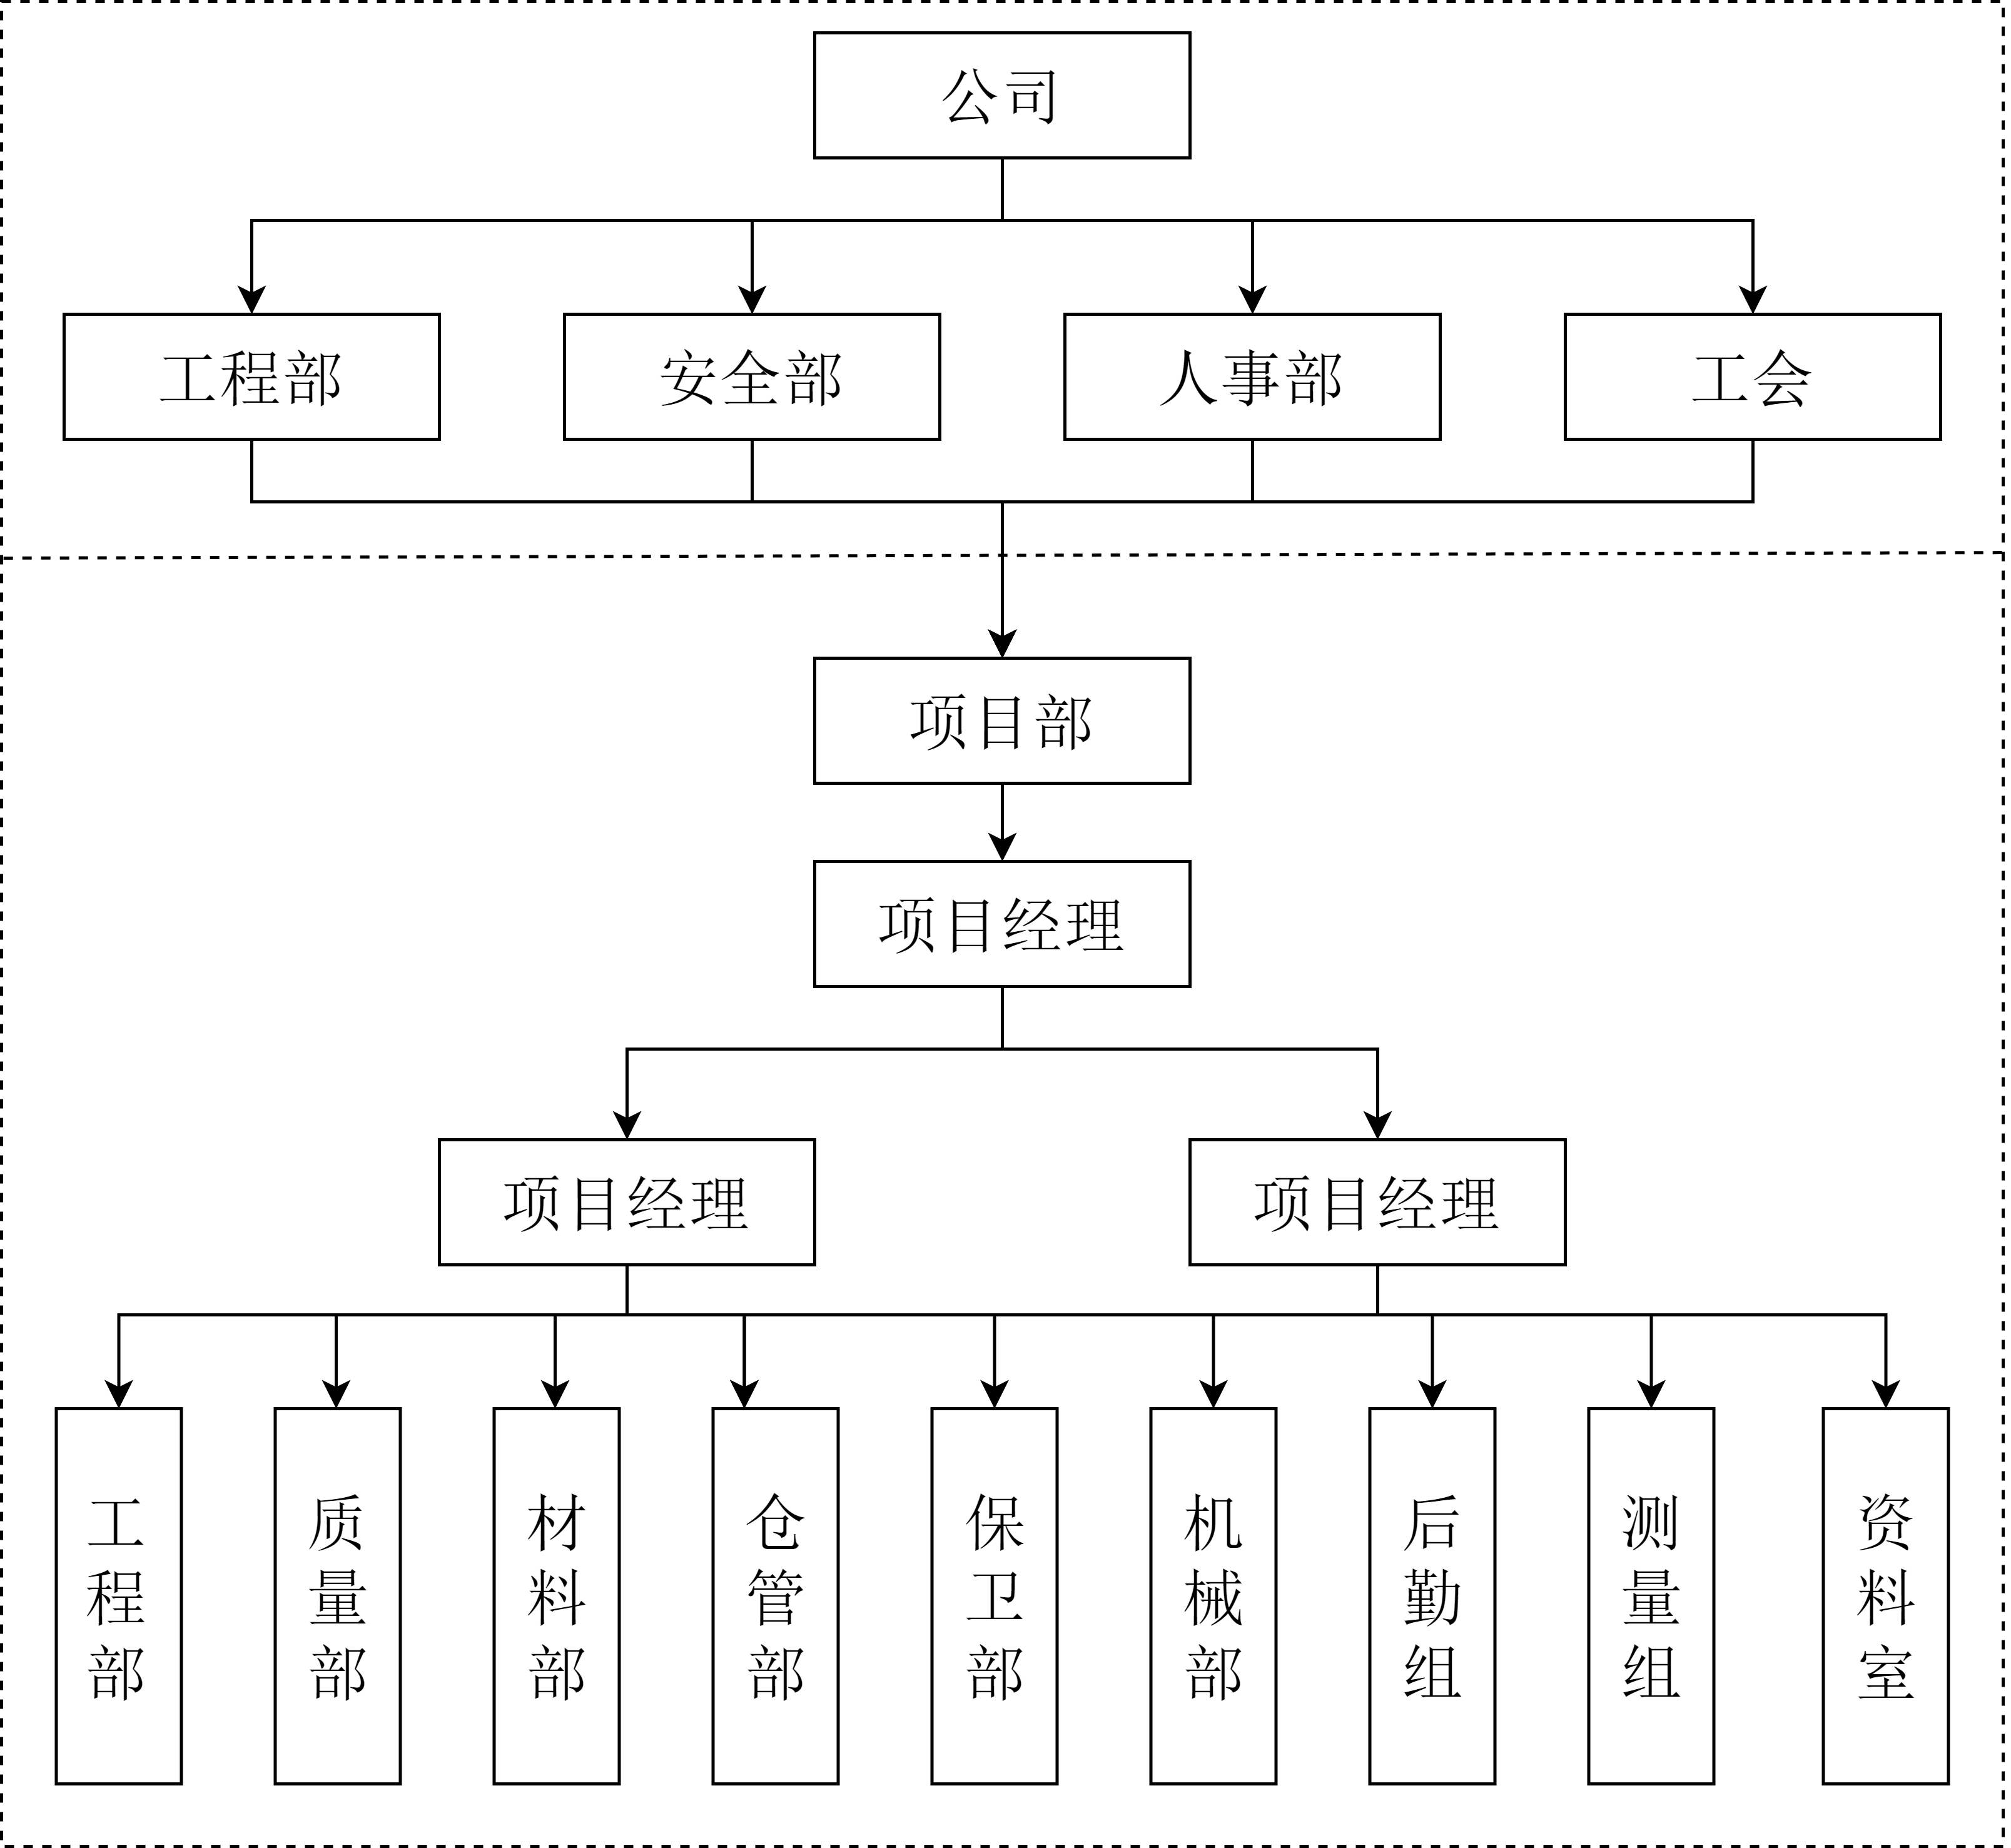
\includegraphics[width=0.8\linewidth]{figure/c2f1.png}
    \caption{施工组织机构图}
    \label{fig:c2f1}
\end{figure}

\subsubsection{主要管理人员职责}

(1) 项目经理岗位职责\\

\quan{1} 全面负责本工程的一切事务,认真贯彻执行《建筑法》、《合同法》和国家有关劳动保护法令和制度以及公司的各项管理制度,
贯彻安全第一、预防为主的方针,按规定搞好安全防范措施,把安全工作落到实处,在各种经济承包中必须包括安全生产、做到讲效益必须讲安全,抓生产首先必须抓安全。

\quan{2} 认真熟悉施工图纸、组织编制施工组织设计方案和施工安全技术措施,组织编制工程总进度计划表和月进度计划表及各施工班
组的月进度计划表。会同项目部相关人员精选强有力的施工队伍,编制工程进度计划及人力、物力计划和机具、用具、设备计划,做到合理组织施工,如发现计划工期无法保证应及时进行调整。

\quan{3} 制定适合本工程项目的管理细则、方案及措施,组织项目部例会,合理安排、科学引导、顺利完成本工程的各项施工任务。
对项目质量全面负责,负责制定质量考核目标,并监督检查。

\quan{4} 对项目成本控制负责,安排、搞好项目的成本核算(按单项和分部分项)单独及时核算,并将核算结果及时通知公司各部门部的管理人员,
以便及时改进施工计划及方案,争创更高效益。及时向各班组下达施工任务书及材料限额领料单。

\quan{5} 对现场文明施工管理负责,组织制定现场文明各项施工管理规定。根据本工程施工现场情况合理规划布局现场平面图,安排、实施、创建文明工地。要求布局合理、经济。

\quan{6} 深入实际了解员工的生活工作学习情况,采纳员工中的合理化建议,妥善解决好施工中出现的各类问题,保质保量顺利完成本工程施工任务。\\

(2) 施工员岗位职责\\

\quan{1} 在项目经理的直接领导下开展工作,贯彻安全第一、预防为主的方针,按规定搞好安全防范措施,把安全工作落到实处,做到讲效益必须讲安全,抓生产首先必须抓安全。

\quan{2} 认真熟悉施工图纸、编制各项施工组织设计方案和施工安全、质量、技术方案,编制各单项工程进度计划及人力、物力计划和机具、用具、设备计划。并监督计划执行情况。

\quan{3} 组织新进场员工技术培训,并做好每道工序的技术交底工作。

\quan{4} 编制文明工地实施方案,根据本工程施工现场合理规划布局现场平面图,安排、实施、创建文明工地。

\quan{5} 编制工程总进度计划表和月进度计划表及各施工班组的月进度计划表,并跟踪实施情况。

\quan{6} 向各班组下达施工任务书及材料限额领料单。配合项目经理工作。\\

(3) 安全员岗位职责\\

\quan{1} 在项目经理领导下,全面负责监督实施施工组织设计中的安全措施、并负责向作业班组进行安全技术交底;

\quan{2} 检查施工现场安全防护、用电安全、机械设施、等是否符合安全规定和标准。如发现施工现场有不安全隐患,应及时提出改进措施,
督促实施并对改进后的设施进行检查验收。对不改进的,提出处置意见报项目负责人处理;

\quan{3} 正确填报施工现场安全措施检查情况的安全生产报告,定期提出安全生产的情况分析报告的意见;

\quan{4} 处理一般性的安全事故;

\quan{5} 按照规定进行工伤事故的登记,统计和分析工作;

\quan{6} 同各施工班组及个人签订安全生产协议书;

\quan{7} 随时对施工现场进行安全监督、检查、指导,并做好安全检查记录。对不符合安全规范施工的班组及个人进行安全教育、处罚,并及时责令整改;

\quan{8} 在安全检查工作中不深入、不细致及存在问题不提出意见又不向上级汇报,所造成的责任事故,应承担全部责任及后果;\\

(4) 质检员岗位职责\\

\quan{1} 在项目经理领导下,负责检查监督施工组织设计的质量保证措施的实施,组织建立各级质量监督保证体系。

\quan{2} 严格监督进场材料的质量、型号、规格、监督各项施工班组操作是否符合规程。

\quan{3} 按照规范规定的分部分项检验方法和验收评定标准,正确进行自检和实测实量,填报各项检查表格,
对不符合工程质量标准、质量要求返工的分部分项工程,写出返工意见并出具罚款单。保证按规定对每一层次、工序不漏检,
并配合施工进度不影响施工。凡经检验不合格的工程,应及时报告项目经理以便采取措施。

\quan{4} 提出工程质量通病的防治措施,提出制订新工艺、新技术的质量保证措施建议。

\quan{5} 对工程的质量事故进行分析,提出处理意见。

\quan{6} 向每个施工班组做(质量验收评定标准)交底。

\quan{7} 每个房间施工都应在施工段(墙、柱、梁、板)贴上质量检查验收表。只有经检验合格才能进入下一工序施工。 \\

\subsubsection{主要管理人员安全生产岗位责任制}

(1) 项目经理安全生产岗位责任制\\

\quan{1} 工程项目经理对工程项目的安全生产负有全面责任

\quan{2} 建立和健全项目体安全管理网络,确定安全管理目标,组织编制安全保证计划

\quan{3} 根据工程特点,加强对分包单位的控制和管理

\quan{4} 认真执行各项安全生产规章制度,明确项目体各管理岗位的安全生产职责,负责检查项目体的安全生产责任制落实情况

\quan{5} 适时组织对工程项目部的安全体系评审和协调

\quan{6} 落实安全保证计划的资源配置

\quan{7} 依据施工组织设计,落实各项安全技术措施,对分部分项工程必须派人进行安全技术交底

\quan{8} 落实专人负责检查特种作业人员持证情况,对新的分包单位进入工地,要有针对地进行安全教育,制止违章操作

\quan{9} 发生工伤事故成立即时组织抢救,保护现场,迅速如实上报,并参加事故调查处理,按“四不放过”的原则,落实各项整改工作

\quan{10} 自觉接受上级安全生产部门的监督和管理\\

(2) 安全员安全生产岗位责任制\\

\quan{1} 贯彻执行劳动保护法规、制度,做好安全生产的宣传,教育和管理工作

\quan{2} 贯彻安全保证计划中的各项安全技术措施,组织参与安全设施、施工用电、施工机械的验收

\quan{3} 对进入现场使用的各种安全用品及机械设备进行各项必要材料的存档及抽查工作

\quan{4} 对分包单位进行安全、消防检查,指导或协助生产负责人解决生产中不安全问题

\quan{5} 参加组织安全、消防活动和安全、消防检查,制止违章作业。对事故隐患开具整改单限期整改并复验,
对有严重险情的有权决定轶作业并及时上报。对违反劳动保护、安全生产法规的行为,经说服劝阻无效时,有权越级上报或举报

\quan{6} 督促有关分包单位做好对新工人、特殊工种人员以及换岗人员的安全技术教育,做好个人安全档案工作

\quan{7} 对施工组织设计中的安全技术措施在实施过程中进行督促检查

\quan{8} 负责对分包单位安全生产的责任考核工作

\quan{9} 参加伤亡事故调查、分析、处理工作。按照“四不放过”的原则,做好安全事故的统计、分析和报告以及归档工作\\

(7) 项目部生产班组长岗位责任制\\

\quan{1} 按照施工方案,组织劳动力进场,彻底做好班组的施工工艺和安全技术措施交底工作

\quan{2} 监督、检查本班组操作工人按图纸、规范、施工方案施工

\quan{3} 组织班组进行自检、互检和交接检工作,发现不合格项目及时组织工人进行整改,确保本班组工作面的质量符合标准

\quan{4} 负责传达项目部的各项管理内容和上报班组各项情况,及时进行调解

\quan{5} 认真遵守安全规章和有关安全生产制度,对本组人员在生产中的安全健康负责

\quan{6} 搞好安全活动日,开好班前、班后安全会,对新调入的工人进行现场班组级安全教育

\quan{7} 组织本班级职工学习施工技术和安全规程及制度,检查执行情况,在任何情况下,均不得违章,不得擅自动用机械、电气、架子等设备

\quan{8} 经常检查施工现场的安全生产情况,加强安全自检,发现问题及时解决,不能解决的采取措施并及时上报

\quan{9} 发生工伤事故要详细记录并及时上报,组织全组人员认真分析,提出防范措施。发生重大伤亡事故要保护现场并立即上报项目部主管\\

\subsection{施工总平面布置说明}
\subsubsection{现场道路}
\subsubsection{现场材料堆放}
\subsubsection{现场垂直运输系统}
\subsubsection{现场用电布置}
\subsubsection{现场临时设施}

\subsection{施工总进度计划及工期保证措施}
\subsubsection{整体工期控制目标}
\subsubsection{主要施工程序进度计划控制}
\subsubsection{工期保证措施}

为确保本工程如期、保质保量地完成,项目部将在以下几个方面采取相应的措施:\\

(1) 施工组织保障措施\\

为保证施工计划完成,我们将选派有丰富的现场施工组织管理经验的、并曾担任过类似工程的项目经理担任该工程项目经理。
以加强项目部管理能力和组织协调能力,及时解决施工中遇到的问题,保证施工中各环节、各专业、各工种之间的协调与平衡。
对工程质量、安全进行监督及人力、财力、物力的统一调度,确保施工顺利进行,杜绝因管理不善造成施工脱节、资源浪费、工期延误现象的发生。\\

(2) 合理的施工方案\\

\quan{1} 充分熟悉本工程的设计图纸,对拟定的施工组织设计、施工方案及方法进行认真的分析比较,作到统筹组织、全面安排,确保总体目标计划。在施工过程中制定阶段性工期控制点,确保按期完工。针对工程特点,采用分段流水施工方法,减少技术间歇,突出重点,制定严密的、紧凑的、合理的施工穿插,尽可能压缩工期,加快施工进度。

\quan{2} 合理地加入投入机械,提高机械化作业程度,充分满足工程所需的人、财、物要求。

\quan{3} 对各班组进行教育,责任到人。各区分段划分负责人,举行施工质量、进度、安全等评比,奖优罚劣。\\

(3) 做好各种资源的供应\\

\quan{4} 根据施工组织设计的要求和施工进度计划中各个阶段控制点的要求,编制劳动力进场计划、材料进场计划、机械设备进场计划、资金使用计划,以保证各种资源能满足施工需要。

\quan{5} 物资材料计划有明确的材料数量、规格和进场时间,现场材料储备应有一定的库存量,以保证工程进度提前或节假日运输困难时工程对物资的需要,确保现场施工正常进行。

\quan{6} 劳动力进场要保证质量,工人进场前必须进行严格的培训和考核。保证足够数量的劳动力。

\quan{7} 按照计划施工机械进场前对机械进行必要的维护、保养和试运转工作,保证所有机械进场后能够投入正常使用。使用期间加强维护与保养,确保机械能正常运行。

\quan{8} 保证足够的资金用于施工,专款专用,确保本工程正常运转。\\

(4) 严格的管理与控制\\

\quan{1} 强化项目方法管理,推行项目方法施工,实行项目经理负责制,设立能协调各方面关系的调度指挥机构,配备素质高、能力强,有开拓精神的管理班子,确保施工进度。

\quan{2} 全面推行计划动态管理,控制工程进度,建立主要形象进度控制点,运用网络计划跟踪技术和动态管理方法,做到周保旬,旬保
月,坚持月平横,周调度、工期倒排,确保总进度的计划实施。

\quan{3} 认真做好施工中的计划统筹、协助与控制。严格坚持落实每周工地施工例会制度,做好每日工程进度安排,确保各项计划落实。
编排详细的工程施工总进度计划,并采用微机管理技术,对施工计划实行动态管理;建立主要工程进度控制点,
围绕总进度计划,编制月、周施工进度计划,作到各分部分项工程的实际进度按计划要求进行;每期根据前期完成情况和其他预测情况变化,
对当期计划和后期计划、总计划进行重新调整和部署,确保按原定或因非施工原因调整了的期限交工。

\quan{4} 实行奖励机制,拟定拿出一定的资金作为目标管理和科技进步奖励基金,充分调动全体施工人员的积极性和创造性,力保各项目标按期实现。

\quan{5} 制定各工序的操作规程和质量标准,强化施工现场管理,做到安全文明施工,努力实现施工管理的标准化、科学化、合理化,使施工有条不紊。

\quan{6} 强化项目部内部管理人员效率与协调,增强与业主的联系,加强对劳务人员的控制和与各供货商的协作,并确保各方及个人的职责分工,
减少扯皮现象,争取将围绕本工程建设的各方面人员充分调动起来,共同完成工期总目标。

\quan{7} 创造和保持施工现场各方面各专业之间的良好的人际关系,使现场各方认清其间的相互依赖和相互制约的关系。特别是加强同交通疏导、
材料运输、周围居民的协调,增进与业主、监理、设计单位的联系和配合,及时解决问题。\\

\subsection{主要项目施工方法和技术措施}
\subsubsection{土方工程}

\begin{itemize}
    \item [1)]场地清理后,即可进行土方开挖,开挖顺序为:按已划分的二个施工流水段分别同时开挖,就地堆积余土。
    \item [2)]基坑开挖按确定的施工顺序逐个采用人工开挖,人工装土,自卸车运土的方式施工。
    \item [3)]根据工程标底的要求:土方开挖为三类土,为保证土壁稳定,开挖时放坡系数暂为 1:0.33 ,由于无现成地质资料参考暂不考虑基坑护壁的支撑。
    \item [4)]土方开挖先测放基坑开挖白线,人工开挖至基底标高后,进行修正清理,测量放线人员准确测放基底标高、轴线、基础的外形尺寸,经自验无误后,做好基坑隐蔽记录,并请监理工程师复核。
    \item [5)]基坑回填采用人工夯实。回填注意控制土含水率,采用同类土填筑,分层回填虚铺厚度每层控制在 30cm 以内,夯实后,干容重不得小于 1.65$\mathsf{g/cm^3}$。
    \item [6)]基坑开挖程序一般是:测量放线 → 切线分层开挖 → 排降水 → 修坡 → 整平 → 留足预留土层等。相邻基坑开挖时,应遵循先深后浅或同时进行的施工程序。挖土应自上而下水平分段分层进行,每层 0.3m 左右,边挖边检查坑底宽及坡度,不够时及时修整,每3m左右修一次坡,至设计标高,再统一进行一次修坡清底,检查坑底宽和标高,要求坑底凹凸不超过1.5m。
    \item [7)]基坑开挖应防止对地基土的扰动。采用机械开挖,为避免破坏基底土,应在基底标高以上预留一层人工清理。
    \item [8)]基坑开挖完后应进行验槽,作好记录,如发现地基土质与地质勘探报告、设计要求不符时,应与有关人员研究及时处理。
\end{itemize}

\subsubsection{钢筋工程}

(1) 钢筋制作\\

钢筋加工制作时,要将钢筋加工下料表与设计图复核,检查下料表是否有错误和遗漏,对每种钢筋要按下料表检查是否达到要求,经过这两道检查后,
再按下料表放出实样,试制合格后方可成批制作,加工好的钢筋要挂牌堆放整齐有序。

施工中如需要钢筋代换时,必须先充分了解设计意图和代换材料性能,严格遵守现行钢筋混凝土设计规范的各种规定,并不得以等面积的高强度钢筋代换低强度的钢筋。
凡重要部位的钢筋代换,须征得设计单位同意,并有书面通知时方可代换。

\quan{1} 钢筋表面应洁净,粘着的油污、泥土、浮锈使用前必须清理干净,可结合冷拉工艺除锈。

\quan{2} 钢筋调直,可用机械或人工调直。经调直后的钢筋不得有局部弯曲、死弯、小波浪形,其表面伤痕不应使钢筋截面减小 5%。

\quan{3} 钢筋切断应根据钢筋号、直径、长度和数量,长短搭配,先断长料后断短料,尽量减少和缩短钢筋短头,以节约钢材。\\


(2)钢筋绑扎与安装\\

钢筋绑扎前先认真熟悉图纸,检查配料表与图纸,设计是否有出入,仔细检查成品尺寸、形状是否与下料表相符。核对无误后方可进行绑扎。
采用 20# 铁丝绑扎直径 12 以上钢筋,22# 铁丝绑扎直径 10 以下钢筋。

\quan{1} 竖向钢筋的弯钩应朝向柱心,角部钢筋的弯钩平面与模板面夹角,对矩形柱应为 45° 角,截面小的柱,用插入振动器时,弯钩和模板所成的角度不小于 15°。

\quan{2} 箍筋的接头应交错排列垂直放置;箍筋转角与竖向钢筋交叉点均应扎牢(箍筋平直部分与竖向钢筋交叉点可每隔一根互成梅花式扎牢)。绑扎箍筋时,铁线扣要相互成八字形绑扎。

\quan{3} 柱筋绑扎时应吊线控制垂直度,并严格控制主筋间距。柱筋搭接处的箍筋及柱立筋应满扎,其余可梅花点绑扎。

\quan{4} 当梁高范围内柱(墙)纵筋斜度 b/a≤1/6 时,可不设接头插筋;当 b/a>1/6 时,应增设上下柱(墙)纵筋的连接插筋,锚入柱(墙)内, \\

(3)质量标准\\

\quan{1} 钢筋的材质。规格及焊条类型应符合钢筋工程的设计和施工规范,有材质及产品合格证书和物理性能检验,对于进口钢材需增加化学性能检定,检验合格后方能使用。

\quan{2} 钢筋的规格、形状、尺寸、数量、间距、锚固长度、接头位置、保护层厚度必须符合设计要求和施工规范的规定。

\quan{3} 焊工必须持相应等级焊工证才允许上岗操作。

\quan{4} 在焊接前应预先用相同的材料、焊接条件及参数,制作二个抗拉试件,其试验结果大于该类别钢筋的抗拉强度时,才允许正式施焊,此时可不再从成品抽样取试件。


\subsubsection{模板及支撑工程}

柱模板安装前,应按设计要求绑扎好柱筋,做好隐蔽记录,按照柱脚轴线及断面尺寸装好柱脚外围拦板,再扶柱板,扶直后先用临时支撑固定,待一列(纵横方向)柱模板装好,
进行中轴线和垂直度校正,校正无误后四周用斜撑钉牢固。

墙自身固定均采用竖向木枋(@≤300)和水平Φ48钢管(间距同螺杆)组成,用 Φ16 螺栓水平钢管对拉以控制截面,螺杆起步间距 ≤250,横向间距为 ≤500mm,竖向间距 ≤500,
楼层上预埋 Φ20@500 的钢筋定位桩以定位并防止墙根部浇混凝土时移位。

外墙模板的空间固定采用顶撑相结合的方法固定,即钢支撑作为压杆,钢丝绳花蓝螺杆作拉杆,压杆与拉杆的间距为 1.8m,内墙模板的空间固定采用钢支撑在墙两侧,
斜向对顶的方法固定。为了防止外墙根部上下层接头位置胀模,上层模板应落下并低于下层楼面不小于 300,并支撑于架设在下层柱顶预埋螺栓上的枋木面上。

附墙柱用胶合板,自身固定用坚向木枋和水平钢管,Ф16 对拉螺杆控制截面(竖向 @≤500)。墙柱支模前根据楼层放线先用 30 宽 18 厚胶全板条在砼楼面上钉出墙模板位置,
这样既便于柱模板定位准确,又便于加强柱模板根部固定,防止柱根部混凝土漏浆。

对通排柱模板,应先装两端柱模板,校正固定,拉通长线校正中间各柱模板。

对截面大于	400mm 的柱,用螺栓或钢筋箍收紧柱模木枋,以不鼓突、不漏浆为准。安装柱模时应在下脚留清扫口。


\subsubsection{混凝土工程}

(1) 浇筑的一般要求\\

\quan{1} 浇筑前应对模板浇水湿润,柱模板的清扫口应在清除杂物及积水后再封闭。

\quan{2} 混凝土自吊斗口下落的自由倾落高度不得超过 2 米,如超过 2m 时必须采取加串筒措施。

\quan{3} 浇筑竖向结构混凝土时,如浇筑高度超过3m时,应采用串筒、导管、溜槽或在模板侧面开门子洞。

\quan{4} 浇筑混凝土时应分段分层进行,每层浇筑高度应根据结构特点、钢筋疏密决定。一般分层高度为插入式振动器作用部分长度的 1.25 倍,大不超过 500mm,平板振动器的分层厚度为 200mm。

\quan{5} 使用插入式振动器应快插慢拔,插点要均匀排列,逐点移动,按顺序进行,不得遗漏,做到均匀振实。移动问距不大于振动棒作用半径的 1.5 倍(一般为 300\textasciitilde400mm)。
振捣上一层时应插入下层混凝土面 50mm,以消除两层间的接缝。平板振动器的移动间距应能保证振动器的平板覆盖已振实部分边缘。

\quan{6} 浇筑混凝土应连续进行。如必须间歇,其间歇时问应尽量缩短。并应在前层混凝土初凝之前,将次层混凝土浇筑完毕。问歇的最长时间应按所有水泥品种及混凝土初凝条件确定
一般超过 2 小时应按施工缝处理。

\quan{7} 浇筑混凝土时应派专人经常观察模板钢筋、预留孔洞、预埋件、插筋等有无位移变形或堵塞情况,发现问题应立即停止浇灌,并应在已浇筑的混凝土上初凝前修整完毕。

\quan{8} 混凝土浇筑前准确掌握天气情况,避开雨天,尽量安排混凝土在夜间浇筑,以降低较厚处混凝土内部水化热。浇注混凝土时,模板、钢筋、应设专人值班,如有位移、变形应及时处理,确保混凝土质量。\\

(2) 梁、板、柱混凝土浇筑方法\\

\quan{1} 柱、墙浇筑前,或新浇混凝土与下层混凝土结合处,应在底面上均匀浇筑 50mm 厚与混凝土配比相同的水泥砂浆。砂浆应用铁铲入模,不应用料斗直接倒入模内。

\quan{2} 柱、墙混凝土应分层浇筑振捣,每层浇筑厚度控制在 500mm 左右。混凝土下料点应分散布置循环推进,连续进行;构造柱混凝土应分层浇筑,每层厚度不得超过 300mm。

\quan{3} 浇筑墙体洞口时,要使洞口两侧混凝土高大体一致。混凝土振捣要均匀密实,特别是墙厚较小,门窗洞口结构加筋与连接交错钢筋较密的部位,应采用 Φ25 振动棒,
其它墙梁部位采用 Φ50 振动棒,考虑到墙窗洞下墙体位混凝土封模后无法直接振捣,可事先将窗洞下口留成活口,待混凝土浇至该位置并振捣密实后再行封模和加固。
振捣时,振动棒应距洞边 300mm 以上,并从两侧同时振捣,以防止洞口变形。大洞口下部模板应开口并补充振捣。

\quan{4} 肋形楼板的梁板应同时浇筑,浇筑方法应由一端开始用" 赶浆法"推进,先将梁分层浇筑成阶梯 ,当达到楼板位置时再与板的混凝土一起浇筑。

\quan{5} 楼板浇筑的虚铺厚度应略大于板厚,用平板振动器垂直浇筑方向来回振捣。注意不断用移动标志或插杆检查以控制混凝土板厚度。振捣完毕,用刮尺或拖板抹平表面。

\quan{6} 在浇筑与柱、墙连成整体的梁和板时,应在柱和墙浇筑完毕后停歇 1\textasciitilde1.5 小时,使其获得初步沉实,再继续浇筑。

\quan{7} 施工缝设置:宜沿着次梁方向浇筑楼板,施工缝应留置在次梁跨度 1/3 范围内,施工缝表面应与次梁轴线或板面垂直。单向板的施工缝留置在平行于板的短边的任何位置。

\quan{8} 施工缝应用木板、钢丝网挡牢。施工缝处须待已浇混凝土的抗压强度不少于 1.2MPa 时,才允许继续浇筑。

\quan{9} 在施工缝处继续浇筑混凝土前,混凝土施工缝表面应凿毛,清除水泥薄膜和松动石子,并用水冲洗干净。排除积水后,先浇一层水泥浆或与混凝土成分相同的水泥砂浆然后继续浇筑混凝土。\\

(3) 楼梯混凝土浇筑\\

\quan{1} 楼梯段混凝土自下而上浇筑。底板混凝土与踏步混凝土一起浇筑,不断连续向上推进。

\quan{2} 楼梯混凝土宜连续浇筑完成。

\quan{3} 施工缝位置:根据结构情况可留设于楼梯平台板跨中或楼梯段 1/3 范围内。 \\

(4) 混凝土的养护\\

\quan{1} 混凝土浇筑完毕后,应在 12 小时以内加以覆盖,并浇水养护。

\quan{2} 混凝土浇水养护日期,掺用缓凝型外加剂的混凝土不得小于 14 天。在混凝土强度达到 1.2MPa 之前,
不得在其上踩踏或施工振动。柱拆模后,用棉布包住,浇水在棉花布上养护,以确保立面结构表面保持湿润状态。

\quan{3} 每日浇水次数应能保持混凝土处于足够的润湿状态。


\subsubsection{脚手架工程}

(1)  钢管采用外径 48mm、壁厚 3.5mm 的焊接钢管,也可采用同样规格的无缝钢管或外径 51mm 、壁厚 3mm 的焊接钢管,钢管材质宜使用力学性能适中的 Q235 钢,
其材性应符合《碳素结构钢》(CB700—88)的相应规定。用于立杆、大横杆、剪力撑和斜杆的钢管长度为 4~6.5m,用于小横杆的钢管长度为 1.8~2.2m,以适应脚手架宽的需要。

(2)  作为脚手架杆件使用的钢管必须进行防锈处理:即对购进的钢管先行除锈,然后内壁擦涂两道防锈漆,处壁涂防锈漆一道和面漆两道。
在脚手架使用一段时间以后,由于防锈层会受到一定的损伤,因此需重新进行防锈处理。

(3)  扣件式脚手架的作业层面可根据所用脚手板的支承要求设置横向平杆,因而可使用各种形式的脚手板。

(4) 对脚手板的技术要求为:

\quan{1} 脚手板的厚度不宜小于 50mm,宽度不宜小于 200mm,重量不宜大于 30kg;
\quan{2} 确保材质符合规定;
\quan{3} 不得有超过允许的变形和缺陷。


\subsubsection{砌体工程}

(1) 砌筑砖砌体时,砖应提前1—2d浇水湿润,含水率宜为10—15\%。

(2) 砖墙砌筑应上下错缝,内外搭砌,灰缝平直,砂浆饱满,水平灰缝厚度和竖向灰缝宽度一般为 10mm,但不应小于 8mm,也不应大于 12mm。

(3) 砖墙的转角处和交接处应同时砌筑,均应错缝搭接,所有填充墙在互相连接、转角处及与混凝土墙连接处均应沿墙高设置 2Φ6@500 通长拉结筋。
对不能同时砌筑而又必须留置的临地问断处应砌成斜槎。如临时间断处留斜槎确有困难时,除转角处外,也可留直槎,但必须做成阳槎,
并加设拉结筋,拉结筋的数量按每 12cm 墙厚原放置一根直径 6mm 的钢筋,间距沿墙高不得超过 50cm,埋入长度从墙的留槎处算起,每边均不应小于50cm,未端应有90° 弯钩。

(4) 隔墙和填充墙的顶面与上部结构接触处用侧砖或立砖斜砌挤紧。
